% High throughput experimentation
The advent of high-throughput experiments holds the prospect of significantly accelerating the speed of materials discovery\cite{Liu2019}. The synthesis and characterization of novel materials are becoming increasingly efficient and automated, increasing the throughput of samples in experimentation pipelines\cite{MacLeod2019, Ludwig2019, Ozaki2020}.

% On Rietveld refinement
After fabricating a new material, a number of analysis techniques can be used to characterize the sample. One method that can be used for phase identification, phase quantification, grain size characterization, and to determine the crystal structure of a new material is powder X-ray diffraction (pXRD). 
When using pXRD measurements, crystal structures are typically determined through Rietveld refinement. In Rietveld refinement, an initial crystal structure model is fitted to the observed diffractogram by iteratively updating the structural model. Each update of the structural model seeks to minimize the difference between the observed diffractogram and the diffractogram simulated from the current structural model \cite{Dinnebier2019, Cano2021}. As Rietveld refinement is a local optimization method, the result of the refinement procedure is generally only as good as the initial structural model the process started from.

% Manual rietveld refinement and its problems
Manually performing Rietveld refinement is time-consuming and often requires expert knowledge. It is not scalable to the degree required to keep up with advances in throughput and efficiency in other steps of the experimentation pipeline. The refinement process requires the operator to determine an initial structural model from which the refinement can start and as well as initial values for parameters that characterize the background \cite{mccusker1999}. The structural model is usually obtained using search-match software, which identifies crystal structures with similar powder diffraction patterns from a database of crystal structures with accompanying powder diffraction patterns. However, an initial structural model obtained from such a database is not guaranteed to lead to an accurate structure solution through Rietveld refinement, especially not for novel structures. Additionally, attempting to refine all crystal structure parameters at once is known to lead to unphysical results\cite{Ozaki2020}. Hence parameters are refined iteratively, with each iteration only refining a limited set of parameters. Finding the correct order in which to refine structure parameters and finding the correct values for initial background parameters both present problems that add to the difficulty of the refinement process.

% Simulated pattern machine learning successes + Sim/Exp performance gap
Machine learning has the potential to speed up the manual analysis of powder diffractograms and keep pace with an automated high-throughput experimentation environment\cite{Agrawal2019, Surdu2023}.
Models can be either trained to predict crystal structure information directly given a diffractogram, or they can be used to automate the conventional refinement workflow. In the latter case a model would first predict an initial crystal structure \cite{Surdu2023} which is then refined by a second model trained to perform the refinement process \cite{Feng2019}. So far due to an absence of labeled datasets with experimental diffractograms\cite{Wang2020}, machine learning in this domain has largely relied on diffractograms simulated from known structures\cite{Park2017, Lee2023} or, most recently, from generated synthetic crystals\cite{Schopmans2023}. 
Models trained on datasets with simulated diffractograms have already shown strong performance in predicting phases \cite{Park2017,chenAutomatingCrystalstructurePhase2021, changProbabilisticPhaseLabeling2023}, lattice parameters\cite{Dong2021, Chitturi2021, Habershon2004, zhang2024crystallographic}, spacegroup \cite{cao2024simxrd, Schopmans2023, Oviedo2018, Park2017, Vecsei2018, Zaloga2020, Suzuki2020, Chakraborty2021,zhang2024crystallographic}, and crystallite size \cite{Dong2021, Chakraborty2021} from simulated diffractograms.
However, the performance substantially drops off when these models are applied to data originating from experiments \cite{cao2024simxrd, Schopmans2023,zhang2024crystallographic, Wang2020, Vecsei2018}. This discrepancy in performance arises due to imperfections in experimental data which are not present in diffraction patterns modeled under ideal conditions. This is discussed in more detail below.

Both labeled and unlabeled datasets of experimental powder diffractograms hold significant value for machine learning-based pXRD analysis, particularly with regard to bridging the performance gap between simulated and experimental domains. Labeled experimental data can be used to test and benchmark existing and new automated analysis approaches. This enables researchers to gauge how well a given model would perform under real-world conditions if integrated into an automated experimentation pipeline. Unlabeled experimental data enables machine learning researchers to evaluate how closely their simulations represent experimental data and modify their simulation algorithms accordingly. Unlabeled data can also find applications in transfer learning approaches to transfer model capabilities from the domain of simulated diffractograms to the domain of experimental diffractograms. While some experimental powder databases exist, their utility is limited by the fact that they are either small or not openly accessible.

In this work, we introduce an open powder X-ray diffraction (opXRD) database featuring a broad range of patterns collected from experiments.\added{The objective of this work is to introduce and disseminate a large, open experimental pXRD dataset, paving the way for future studies that will evaluate and benchmark its impact on model performance.} With a total of $\numpatterns$ patterns collected from 6 contributing institutions, the opXRD database exceeds the size of the previously largest database of openly accessible experimental powder diffraction data by two orders of magnitude. To the best of our knowledge, the largest database of this type is the RRUFF database, containing 1290 experimental powder diffraction patterns \cite{lafuente2015}. Larger commerical datasets such as the PDF5+\cite{GatesRector2019} and the Linus Pauling File\cite{villars2018} exist, but their utility is limited by fees and restrictive licenses. License terms of commercial datasets, such as the PDF5+ and the Linus Pauling File, prohibit or restrict the publication of models trained on their data. In contrast, the opXRD database is both free and imposes no restrictions on how its data is used. Fig.~$\eqref{fig:ml_uses}$ provides an overview of machine learning workflows enabled and supported by the opXRD database.

% VISUAL ABSTRACT FIGURE
\begin{figure}[!htb]
    \centering
    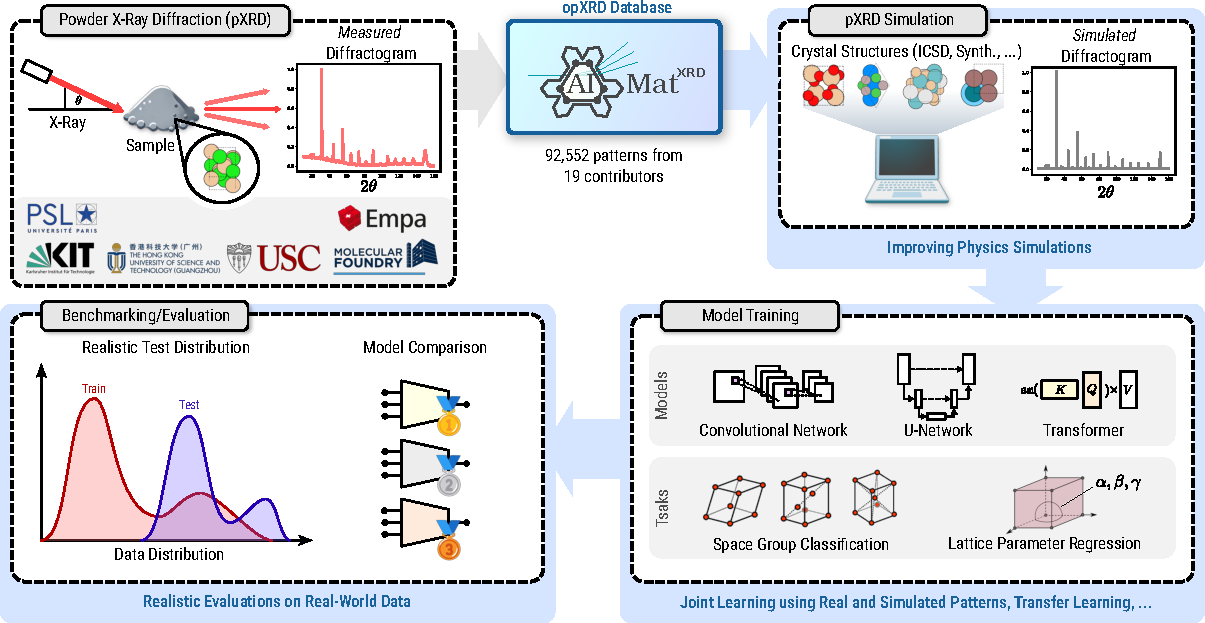
\includegraphics[width=1.0\linewidth]{figures/pipeline.pdf}
    \caption{Experimental powder X-ray diffraction (pXRD) patterns from several contributors are collected in the \textit{opXRD} database. The proposed open-access database of experimental data aims to support each step in the pXRD-related machine learning workflow by informing better physics simulations, supplying model training data, and providing a foundation for realistic performance evaluations.}
    \label{fig:ml_uses}
\end{figure}

Of the $\numpatterns$ patterns in the opXRD database\added{,} \numlabeled patterns come with at least partial structural information of the underlying sample. Of these \numlabeled labeled patterns, \numfull have \replaced{labels of the full crystal structure}{full structural labels including atomic coordinates}. \deleted{This constitutes an experimental pXRD test dataset that is larger in size, richer in labels, and broader in represented experimental setups than the RRUFF database, which only provides lattice parameters as labels\cite{Armbruster2015}.} 
\added{While the fraction of samples with structural labels (\SI{2.35}{\percent}) may appear small, this fraction represents the largest openly available collection of experimentally derived, structure-annotated pXRD patterns. As a comparison, the RRUFF database, often used for benchmarking ML models, contains partial labels for \num{1290} patterns, but no atomic coordinates. The pXRD dataset is larger in size, richer in labels, and broader in represented experimental setups compared to previous openly available datasets. Given the inherently labor-intensive nature of manual labeling in pXRD analysis, it is impractical to expect a fully labeled dataset at the scale of simulated training datasets, which commonly exceed $10^6$ patterns \cite{Salgado2023, Schopmans2023}. Therefore, next to the option of benchmarking models and methods on the labeled subset, opXRD is designed to complement vast simulated datasets. This can be achieved through the adjustment of simulation parameters by comparing with the unlabeled fraction of the dataset, and through transfer learning strategies.
We now want to discuss these two options of utilizing the unlabeled portion of our dataset in more detail.}
\deleted{However, since the majority of the opXRD database is unlabeled we also want to further discuss the uses of unlabeled data, including its role in improving pattern simulations and its application in transfer learning approaches.}

The neglected effects that lead to discrepancies between simulated patterns and patterns stemming from experiments are largely known. Unaccounted effects may include preferred crystallite orientation, variations in grain size, crystal defects, the impact of temperature on the scattering process, internal stress, the non-monochromaticity of the X-ray source, and X-ray-induced fluorescence\cite{cao2024simxrd, Waseda2011, Pecharsky2023}. Additionally, varying experimental setups produce distinct powder diffraction patterns on the same sample. Features that may vary between experimental setups include the shape of diffraction peaks, the wavelength and polarization of the employed X-ray source, and the detector geometry \cite{cao2024simxrd, Waseda2011, Pecharsky2023}. The recorded scattering angles may also be slightly falsified if the sample is displaced from its intended position\cite{cao2024simxrd,hulbert2023}. As these and more neglected effects are integrated into the simulation process, real powder diffraction data can be used to evaluate how closely simulated data matches up with real data. While direct comparisons are only possible on labeled patterns, comparing the strength and prevalence of features between simulated and real data can nevertheless provide information about the fidelity of the simulation. Taking into account all neglected effects without making approximations will incur significant computational costs that will lower the size of the generated training data. A more efficient approach could be to use real experimental data to identify the effects that have the largest impact in practice and model them heuristically.

The second way in which unlabeled experimental data can serve to bridge the performance gap between simulated and experimental domains is through transfer learning. The objective of transfer learning is to transfer the capabilities of a model learned on a source domain in which labeled data is abundant to a target domain in which labeled data is sparse\cite{Zhuang2021}. In this context, the source domain is simulated powder diffraction patterns and the target domain is experimental powder diffraction patterns. Many approaches to transfer learning have been proposed, particularly in the domain of image classification \cite{Gatys2016, Ganin2015}.  These existing techniques can be adapted to facilitate transfer learning in the context of pXRD patterns. Seddiki \textit{et al}. have already successfully applied transfer learning in the domain of mass spectrometry to boost the accuracy of mass spectrum classification models\cite{Seddiki2020}. Since both mass spectrometry data and pXRD data are one-dimensional, this work demonstrates the merit of transfer learning in a setting similar to pXRD.

% Contributing + community driven
The opXRD database is intended as a growing, community-driven initiative. The database we present here is the first version, but we hope to further increase the database size through active engagement with the pXRD community. Our primary objective is to minimize the effort and thus the barrier to contributing experimental data to the opXRD database. Thus, we developed a program that helps to find and share data from pXRD lab computers. Users can select their most common pXRD file types, the program lists all files of that type, and users can select or deselect certain folders or files for sharing. Selected contributions will be uploaded to opXRD, processed to a common file format, and---if wanted---published on Zenodo on behalf of the contributors, before becoming part of the opXRD database. If labels are available, they can be shared with opXRD as well. Further details can be found on the opXRD website (\url{https://xrd.aimat.science/}). An overview of this process is given in Fig.~$\eqref{fig:submission}$ below.

\begin{figure*}[!htb]
    \centering
    \includegraphics[width=\linewidth]{figures/overview.pdf}
    \caption{Overview of the data collection pipeline. Datasets are submitted using an online submission form, optionally with the help of our submission helper software. After post-processing and data homogenization, we offer the creation of a Zenodo entry for each user submission and subsequently include the submission in the opXRD database.}
    \label{fig:submission}
\end{figure*}

As argued by Aranda and Kroon-Batenburg \textit{et al}.\cite{Aranda2018, Kroon-Batenburg2024}, sharing raw powder diffraction data is not only in the interest of furthering machine learning research but is also in line with open science principles. It furthers the ability of other researchers to reproduce published work and in turn, adds to the credibility of the publisher of the data. Compared to publishing data individually, publishing data on the opXRD database has the added benefit of contributing to a large, homogenous dataset with a standardized interface. This makes the data more easily accessible to other researchers and provides more value to researchers seeking large quantities of data. However, further data annotation with metadata is required to fully fulfill the FAIR data principles.

The opXRD database contains pXRD patterns from single and multiphase materials from a wide variety of material classes, including high-entropy materials, perovskites, and commercial catalysts. Some of the XRD data was collected on thin-films rather than on true powder samples, which may influence the quality of the data in regards to full structure resolution. Additionally, some of the data was collected in grazing-angle geometry rather than in the usual Bragg-Brentano geometry employed in powder diffraction.
The broad range of available experimental samples contained in the opXRD v1.0 database makes it possible to apply state-of-the-art ML approaches to the domain of pXRD analysis. We hope that the opXRD database can drive ML research in this field towards more advanced automated analysis workflows that can accelerate materials science research through ready application in high-throughput experimentation pipelines. Details of the experiments of research groups contributing to the opXRD database are discussed in Section~$\eqref{sec:our_dataset}$. A detailed description of how to acquire and use opXRD data is given in Section~$\eqref{sec:how_to_use}$, and Section~$\eqref{sec:summary_and_outlook}$ describes how further data can be contributed.